In this section, we extend the analysis and results to observe the behavior of IMEX ADER and DeC methods onto the advection-dispersion equation
\begin{equation}
\label{eq: A-Disp_equation}
u_t(x,t) + au_x(x,t) + \beta u_{xxx}(x,t) = 0, \quad a\ge0, \ \beta \ge 0.
\end{equation}
\subsection{FD discretization}
\label{sec: disp_spatial_discretization}
\PO{First, we  introduce at this point the considered spatial discretizations for the advection-dispersion equation. Thereby, we consider the same discretization for the advection term, as introduced in Section~\ref{sec: spatial_discretization}}.\\
For the dispersion term, we will take two different types of methods into account: Central finite difference and upwind schemes. The underlying theory and assumptions are the same as we saw previously and their orders can be proven analogously. We consider the following central finite difference scheme of order $2$ 
\begin{equation}
	\label{eq: CFD-schemes_third_deriv}
	\partial_{\Delta x}^3(u(x_j)) = \frac{1}{{\Delta x}^3}\left(-\frac{1}{2}w_{j-2} + w_{j-1} - w_{j+1} + \frac{1}{2}w_{j+2}\right)
\end{equation}
and the upwind scheme used in \cite{TanChenShu_ImEx_Stability} to test stability for the advection-dispersion equation \eqref{eq: A-Disp_equation}. It is of order 3 and given by
\begin{equation}
\label{eq: shu_upwind_dispersion}
\partial_{\Delta x}^3(u(x_j)) =\frac{1}{4{\Delta x}^3}\left( -w_{j-2} - w_{j-1}  + 10w_{j} - 14w_{j+1} + 7w_{j+2} - w_{j+3}\right).
\end{equation}
For higher orders, we have used stencils of the type $[-r,r+1]$ with the tool \PO{provided in \cite{fdcc}.}
\subsection{von Neumann analysis}
As done previously, we will perform von Neumann analysis by looking at the coefficients of the finite difference schemes, i.e.,
$$C=a\frac{\Delta t}{\Delta x},\qquad P= \beta\frac{\Delta t}{{\Delta x}^3}.$$
So technically, we compute the methods in the same way and just adapt the spatial schemes from the diffusion term to the dispersion term. Remark that also the sign of this term gets changed. 
\subsubsection{Displaying stability}
To denote the considered methods, we use again the notation introduced for the advection-diffusion equation
	\begin{equation*}
[\TMM,\NODES,N, A_n,B_m],
\end{equation*}
where $B_m$ refers to the central finite difference stencil \eqref{eq: CFD-schemes_third_deriv} for $m=2$ and to the upwind third order stencil \eqref{eq: shu_upwind_dispersion} for $m=3$.
We proceed by utilizing the experience of section~\ref{sec: advection_diffusion}, and evaluate the amplification factor 
\begin{equation*}
G(k,\Delta x, \Delta t, a, \beta)=g(k,C,P)
\end{equation*}
to observe where we are stable in dependence of $C$ and $P$. 
In opposition to the advection--diffusion case, in \cite{TanChenShu_ImEx_Stability} only a CFL condition is found, even if, numerically, they observe larger stability regions with a little of dispersion.
We want to give a more comprehensive study of this behavior for different schemes and, as before, we look for meaningful coefficients that bounded by some constants give the stability. 
To find such coefficients, we proceed with an example.
\begin{example}\label{exa: disp_displaying_stability}
	In Figure~\ref{fig: disp_IIMEXDeC2/3} we display the stability areas for the $[\DeC, \eq,2,A_1, B_2]$ and $[\DeC, \eq,3,A_1, B_2]$ on the $C-P$ plane (left figures).
	In the IMEXDeC2 case, we note that for low $P$ a CFL constraint $C\leq 1$ guarantees stability, while for large $P$ we see a linear constraint of the type $P\gtrsim E_0 C $.
	In the IMEXDeC3 case, there is a further unstable region close to the $C=0$ axis. This extra unstable region is due to the fact that IMDeC3 is not A-stable and, hence, for low values of $C$ not enough numerical dissipation is brought to the system.
	
	Anyway, the linear constraint on the large $P$ motivates the following definition of 
	\begin{equation*}
		E_P:=\frac{C}{P}=\frac{\Delta ta}{\Delta x}\frac{\Delta x^3}{\beta\Delta t}=\frac{a \Delta x^2  }{\beta }.
	\end{equation*}
	Now, looking at the right plot for IMEXDeC2 in Figure~\ref{fig: disp_IIMEXDeC2/3}, we observe that either $C\leq 1$ or $E_P\leq E_0 \approx 0.007$ guarantee stability. 
	This is a peculiar result as $E_P=\frac{a  }{\beta \Delta x^2 }$ does not depend on the time discretization.
	The same does not hold of IMEXDeC3, where this area is stable only for large values of $C$, which leads to very inaccurate schemes, as we need $E_P$ small enough, i.e., $\Delta x$ large enough and $C$ large enough, which implies $\Delta t$ even larger.
	Moreover, for the IMEXDeC3 the $E_0$-border is much smaller  than order 2, so the stable region is even tighter for large $C$.
	\begin{figure}
		\centering
		\begin{minipage}[t]{0.32\textwidth}
			\centering
			\includegraphics[width=\textwidth]{pdf/pdepics/disp/contourf_adv_disp_IMEXDeC_gaussLobatto_2_disp_CFD_adv_1_CP.pdf}
			IMEX DeC2 ($C$ vs $P$)
		\end{minipage}
		\begin{minipage}[t]{0.32\textwidth}
		\centering
		\includegraphics[width=\textwidth]{pdf/pdepics/disp/contourf_adv_disp_IMEXDeC_gaussLobatto_2_disp_CFD_adv_1_CE.pdf}
		IMEX DeC2 ($C$ vs $E_P$)
		\end{minipage}
		\begin{minipage}[t]{0.32\textwidth}
		\centering
		\includegraphics[width=\textwidth]{pdf/pdepics/disp/contourf_adv_disp_IMEXDeC_gaussLobatto_2_disp_CFD_adv_1_CE_zoom.pdf}
		IMEX DeC2 ($C$ vs $E_P$, log)
		\end{minipage}\\
		\begin{minipage}[t]{0.32\textwidth}
			\centering
			\includegraphics[width=\textwidth]{pdf/pdepics/disp/contourf_adv_disp_IMEXDeC_equispaced_3_disp_CFD_adv_1_CP.pdf}
			IMEX DeC3 ($C$ vs $P$)
		\end{minipage} 
		\begin{minipage}[t]{0.32\textwidth}
			\centering
			\includegraphics[width=\textwidth]{pdf/pdepics/disp/contourf_adv_disp_IMEXDeC_equispaced_3_disp_CFD_adv_1_CE.pdf}
			IMEX DeC3 ($C$ vs $E_P$)
		\end{minipage}
		\begin{minipage}[t]{0.32\textwidth}
			\centering
			\includegraphics[width=\textwidth]{pdf/pdepics/disp/contourf_adv_disp_IMEXDeC_equispaced_3_disp_CFD_adv_1_CE_zoom.pdf}
			IMEX DeC3 ($C$ vs $E_P$, log)
		\end{minipage}
		\caption{Stability areas for $[\DeC, \eq,2,A_1, B_2]$ and $[\DeC, \eq,3,A_1, B_2]$ with second order central dispersion operator}
		\label{fig: disp_IIMEXDeC2/3}
	\end{figure}
\end{example}
These exemplary stability regions hold for most of the considered cases, i.e. all methods of order 2 do not have the instability areas for small $C$ and large $P$, as well as the IMEX ADER methods with equispaced nodes until order 4 and all IMEX ADER methods with Gauss-Lobatto nodes. 
Remark that these are exactly the methods which seem to be A-stable in their implicit ODE application as discussed in section~\ref{sec: stability_analysis_ODE}. 
All remaining methods possess this unfavorable stability region. 
%Furthermore, it can be observed that for methods corresponding to A-stable implicit ones the instability areas for very small $E_0$ appear for much smaller $E_0$ if the belonging implicit ODE method is A-stable. 
%This can be seen in the previous example and extends to all remaining considered methods.






%Note also that we tested other coefficients, for example $C$ vs $\frac{C^2}{P}$ and did not recognize any favorable restrictions in terms of regularity or borders, as for the advection-diffusion equation. 

\subsubsection{Results for IMEX DeC, sDeC and ADER}
In this section, we present the analysis results as displayed in Example~\ref{exa: disp_displaying_stability}, varying numerical methods. 
We first by testing the schemes of Example~\ref{exa: disp_displaying_stability} with the upwinded third order dispersion discretization.
We have tried increasing the order of (upwinded) dispersion terms without noticing big differences with respect to \eqref{eq: shu_upwind_dispersion}. Hence, we will proceed with the upwind dispersion term $B_3$ introduced in \eqref{eq: shu_upwind_dispersion}.
\begin{example}\label{exa: disp_displaying_stability_upwind}
	In Figure~\ref{fig: disp_IIMEXDeC2/3_GLB_CvsE_upwind}, we display the stability areas for the $[\DeC, \eq,2,A_1,B_3]$ and $[\DeC, \eq,3, A_1,B_3]$ to compare the results to example~\ref{exa: disp_displaying_stability}, in which the only difference is the dispersion term: $B_3$ instead of $B_2$.
	On average, the stability regions increase in this example, in particular $C_0$ is larger, while the small CFL unstable area remains almost unchanged.
%	The $C_0$ borders seem to increase, while we receive a completely different curve shape (again some quadratic-like) for the border of the stable and unstable region in the $C$ vs $P$ view. Also, the unstable regions on the top-left are shrinking even though they do not vanish at all. 
	This shows that also using upwinded dispersion terms we can not resolve the instability for small $C$ and large $P$ for non A-stable schemes.
	\begin{figure}[!h]
		\centering
		\begin{minipage}[t]{0.32\textwidth}
			\centering
			\includegraphics[width=\textwidth]{pdf/pdepics/disp/contourf_adv_disp_IMEXDeC_gaussLobatto_2_disp_Shu_adv_1_CP.pdf}
			IMEX DeC2 ($C$ vs $P$)
		\end{minipage}
		\begin{minipage}[t]{0.32\textwidth}
			\centering
			\includegraphics[width=\textwidth]{pdf/pdepics/disp/contourf_adv_disp_IMEXDeC_gaussLobatto_2_disp_Shu_adv_1_CE.pdf}
			IMEX DeC2 ($C$ vs $E_P$)
		\end{minipage}
		\begin{minipage}[t]{0.32\textwidth}
		\centering
		\includegraphics[width=\textwidth]{pdf/pdepics/disp/contourf_adv_disp_IMEXDeC_equispaced_2_disp_Shu_adv_1_CE_zoom.pdf}
		IMEX DeC2 ($C$ vs $E_P$, log)
		\end{minipage}\\
		\begin{minipage}[t]{0.32\textwidth}
			\centering
			\includegraphics[width=\textwidth]{pdf/pdepics/disp/contourf_adv_disp_IMEXDeC_equispaced_3_disp_Shu_adv_1_CP.pdf}
			IMEX DeC3 ($C$ vs $P$)
		\end{minipage} 
		\begin{minipage}[t]{0.32\textwidth}
			\centering
			\includegraphics[width=\textwidth]{pdf/pdepics/disp/contourf_adv_disp_IMEXDeC_equispaced_3_disp_Shu_adv_1_CE.pdf}
			IMEX DeC3 ($C$ vs $E_P$)
		\end{minipage}
		\begin{minipage}[t]{0.32\textwidth}
			\centering
			\includegraphics[width=\textwidth]{pdf/pdepics/disp/contourf_adv_disp_IMEXDeC_equispaced_3_disp_Shu_adv_1_CE_zoom.pdf}
			IMEX DeC3 ($C$ vs $E_P$, log)
		\end{minipage}
		\caption{Stability areas for $[\DeC, \eq,2,A_1, B_3]$ and $[\DeC, \eq,3,A_1, B_3]$  with third order upwind dispersion operator}
		\label{fig: disp_IIMEXDeC2/3_GLB_CvsE_upwind}
	\end{figure}
\end{example}
%In the following, we will present the stability results for remaining, mentionable cases by looking at the coefficients $C$ vs $E_p$ while using the before considered upwind method for the dispersion term. To distinguish the different orders, we apply the same colors to the bounds as for the advection-diffusion analysis.
%Remark that the colors are assigned to different types of orders, i.e., in one figure to the order of the time-marching method, in another to the order of the advection method.
\begin{figure}
	\centering
	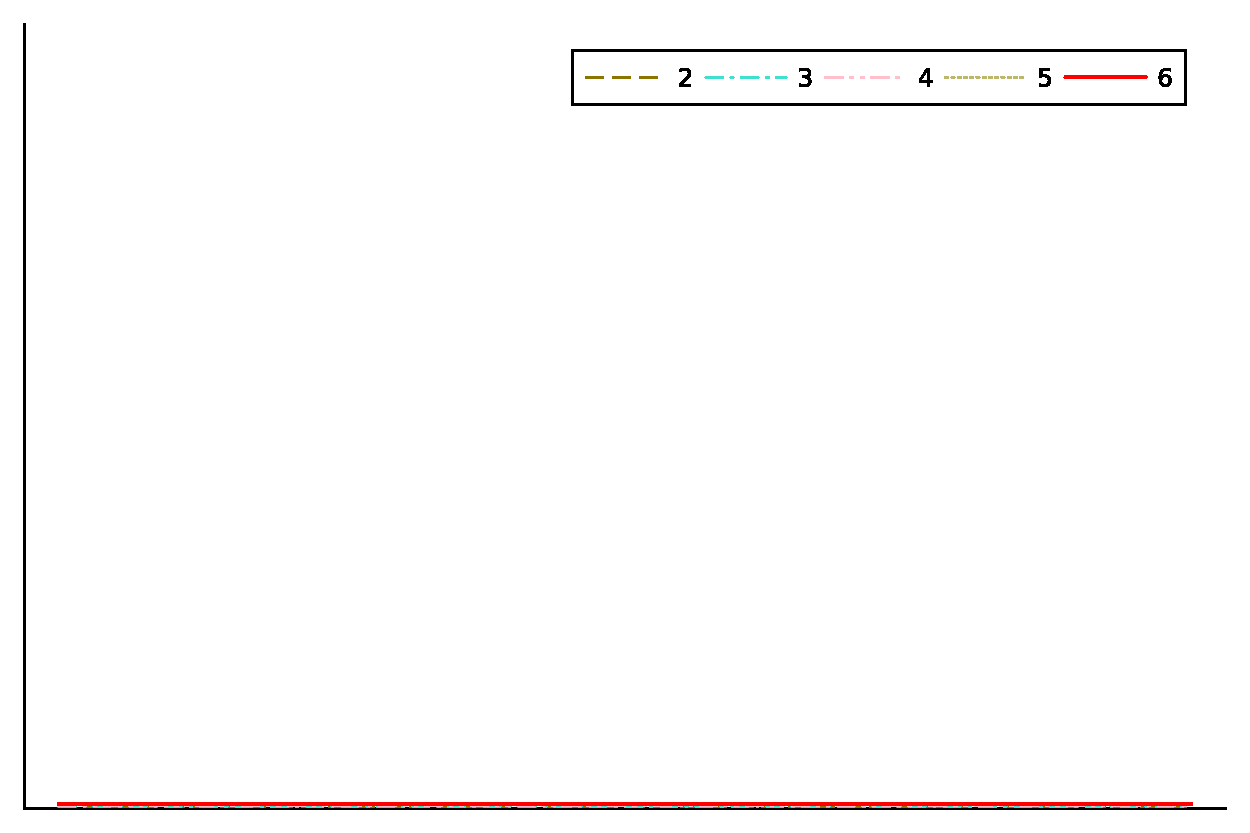
\includegraphics[width=0.4\textwidth,trim={230 340 30 22}, clip]{pdf/pdepics/legends/colors_a-d_new_horiz_2-6_no_order.pdf}\\
	\begin{minipage}[t]{0.32\textwidth}
		\centering
		\includegraphics[width=\textwidth]{pdf/pdepics/disp/IMEXDeC_gaussLobatto_disp_TMM_2-6_newE.pdf}
		\small$[\DeC, \GLB,k, A_1,B_3]$\par
	\end{minipage}
	\begin{minipage}[t]{0.32\textwidth}
		\centering
		\includegraphics[width=\textwidth]{pdf/pdepics/disp/IMEXDeC_subtimesteps_gaussLobatto_disp_TMM_2-6_newE.pdf}
		\small$[\sDeC, \GLB,k, A_1,B_3]$\par
	\end{minipage}
	\begin{minipage}[t]{0.32\textwidth}
		\centering
		\includegraphics[width=\textwidth]{pdf/pdepics/disp/IMEXADER_gaussLobatto_disp_TMM_2-6_newE.pdf}
		\small$[\ADER, \GLB,k, A_1,B_3]$\par
	\end{minipage}\\
	\begin{minipage}[t]{0.32\textwidth}
		\centering
		\includegraphics[width=\textwidth]{pdf/pdepics/disp/IMEXDeC_equispaced_disp_TMM_2-6_newE.pdf}
		\small$[\DeC, \eq,k,A_1,B_3]$\par
	\end{minipage}
	\begin{minipage}[t]{0.32\textwidth}
		\centering
		\includegraphics[width=\textwidth]{pdf/pdepics/disp/IMEXDeC_subtimesteps_equispaced_disp_TMM_2-6_newE.pdf}
		\small$[\sDeC, \eq,k, A_1,B_3]$\par
	\end{minipage}
	\begin{minipage}[t]{0.32\textwidth}
		\centering
		\includegraphics[width=\textwidth]{pdf/pdepics/disp/IMEXADER_equispaced_disp_TMM_2-6_newE.pdf}
		\small$[\ADER, \eq,k, A_1,B_3]$\par
	\end{minipage}
	\caption{Stability areas for orders 2 to 6 with GLB (top) and equi (bottom) nodes, the upwind scheme of \eqref{eq: shu_upwind_dispersion} for the dispersion and an first order backward scheme for the advection term}
	\label{fig: disp_allRK}
\end{figure}

\begin{figure}
	\centering
	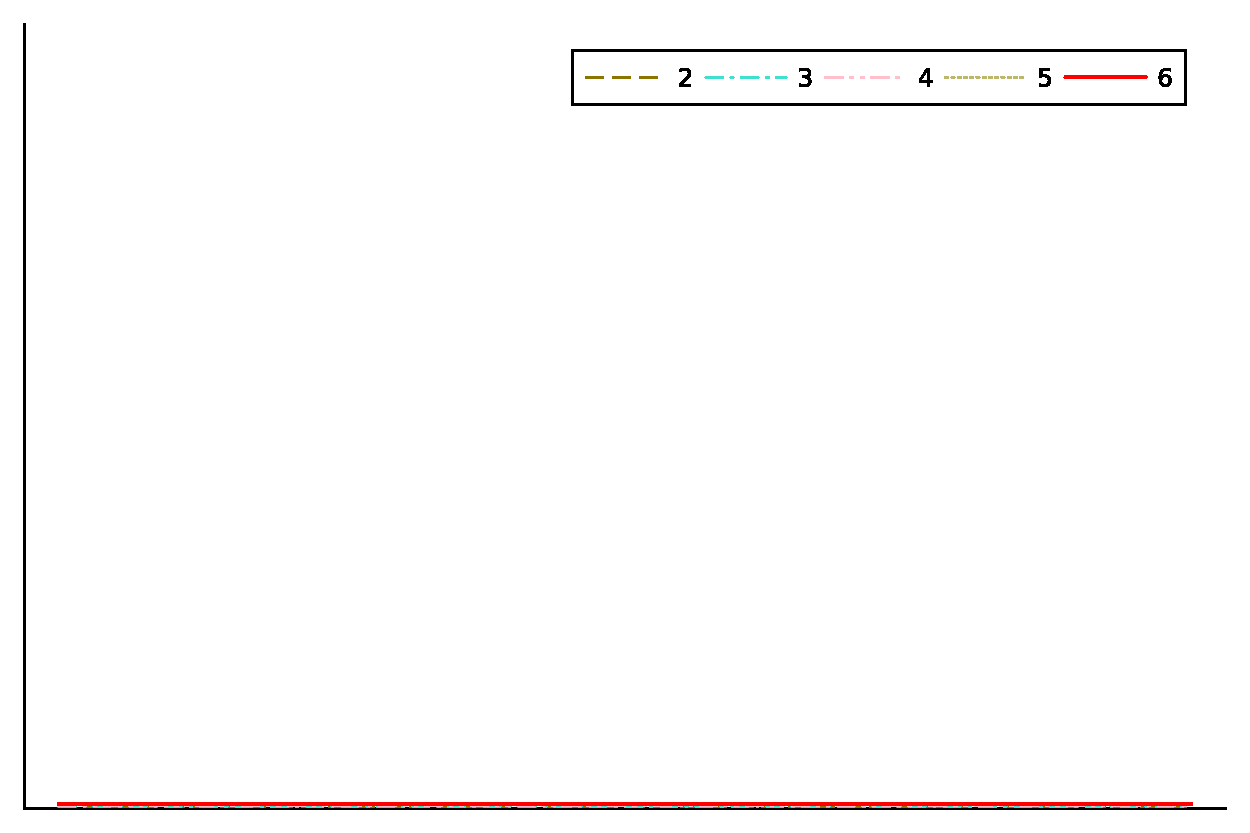
\includegraphics[width=0.4\textwidth,trim={230 340 30 22}, clip]{pdf/pdepics/legends/colors_a-d_new_horiz_2-6_no_order.pdf}\\
	\begin{minipage}[t]{0.325\textwidth}
		\centering
		\includegraphics[width=\textwidth]{pdf/pdepics/disp/IMEXDeC_gaussLobatto_disp_advTMM_2-6_newE.pdf}
		\small$[\DeC, \GLB,k,A_k,B_3]$\par
	\end{minipage}
	\begin{minipage}[t]{0.325\textwidth}
	\centering
	\includegraphics[width=\textwidth]{pdf/pdepics/disp/IMEXDeC_subtimesteps_gaussLobatto_disp_advTMM_2-6_newE.pdf}
	\small$[\sDeC, \GLB,k,A_k,B_3]$\par
	\end{minipage}
	\begin{minipage}[t]{0.325\textwidth}
		\centering
		\includegraphics[width=\textwidth]{pdf/pdepics/disp/IMEXADER_gaussLobatto_disp_advTMM_2-6_newE.pdf}
		\small$[\ADER, \GLB,k,A_k,B_3]$\par
	\end{minipage}
	\caption{Stability areas varying orders 2 to 6 of the advection scheme and time scheme}
	\label{fig: disp_alladv_GLB}
\end{figure}
We proceed now studying the stability regions increasing the order of the time scheme, keeping fixed the advection and dispersion operators ($A_1$ and $B_3$), later on we also increase the accuracy of the advection operator.
In Figure~\ref{fig: disp_allRK}, we can observe the stability regions changing the time scheme order from 2 to 6. 
For DeC methods of order larger than 2, we cannot  not provide bounds that guarantee the stability for small $C$ and $E_P$.
Anyway, away from this area, we observe stable regions for both $C\leq C_0$ with $C_0$ values similar to the ones of the advection--diffusion section, see Table~\ref{tab:CE_values}, and for $E_P\leq E_{P,0}$ with $E_{P,0}\approx 4\cdot 10^{-5}$ independently on the DeC method used.
In general, sDeC guarantees more stability in the region with $C\in [1,10]$ and $C/P\in [10^{-4},10^{-2}]$, while differences between equispaced and GLB are not relevant.

On the other hand, IMEXADER with GLB nodes is very stable and there are clear bounds $C\leq C_0\leq 3$ and $E_P\leq E_{P,0}\leq 10^{-4}$ that guarantee stability. Moreover, there is a large stability area for large $C\leq 10$ and not so small $E_P$.
On the contrary, IMEXADER with equispaced points for order more than 4 is much more unstable and only the are with both $C\leq C_0$ and $E_P \geq E_{P,0}$, which quite restrictive.

Again, the behavior of all these schemes reflects the A-stability property of the corresponding implicit methods.

%values border due to the afore mentioned effects, but a border $C_0\approx 2$ for every method. The same holds for the ADER methods, while we can observe some more unstable behavior for small $E_P$ as $C$ growths. We can also observe smaller borders $C_0$ than for the DeC methods. For the sDeC, we have similar values for $C_0$, while for orders over 2 the border curve seems to be located over some much larger border line $E_{P,0}$ than for the other methods: While DeC and ADER seem to have $E_{P,0}$ border values around $E_p=0.1$, the sDeC has values over 5 for orders over 2, increasing with order. We also note that the anticipated $E_{P,0}$ borders change for different orders and may take similar values as for $E_0$ in the advection-diffusion case. Nevertheless, the minor instability regions below exist as it can be seen in figure~\ref{fig: sDeC4_adv1_upwind_large} for the IMsDeC order 4. For this reason, we can not assign them spatial-independent stability conditions $E_{P,0}$. 

%\begin{figure}[!h]
%	\centering
%	\includegraphics[width=0.48\textwidth]{pdf/pdepics/disp/contourf_adv_disp_IMEXDeC_subtimesteps_gaussLobatto_4_disp_Shu_adv_1_CE.pdf}
%	\caption{The sDeC4 method with GLB nodes displayed on an larger scale.}
%	\label{fig: sDeC4_adv1_upwind_large}
%\end{figure}

%In figure \ref{fig: disp_allRK_EQ}, we show the same methods as before, but using equispaced nodes. We observe no mentionable differences except for the ADER method, where we get different shapes of instabilities for small $E_p$, resulting in $C_0=0$ for order 6.
%This reminds us of the ADER method for the advection-diffusion equation, where we also observed instabilities for higher orders.
%Further, we could observe that the instabilities we obtain for both small $E_p$ and small $C$ are not only small for order 2, but also for higher orders in the ADER case with Gauss-Lobatto nodes and also with equispaced nodes until order 4.  As already mentioned before, this could also be a result of the loss of A-stability for the certain order of the IMADER with equispaced nodes. 



In Figure \ref{fig: disp_alladv_GLB}, we check the stability regions varying the advection and time order of accuracy for DeC and ADER GLB methods. 
We find a loss of stability by increasing the order. We already see a slight reduction of our border $C_0$ for order 2 and 3. Going onto orders 4, 5 and 6, we obtain way larger unstable regions, in particular in the low $E_P$ region that were stable in the only high order in time scheme presented above.

\begin{figure}
	\centering
	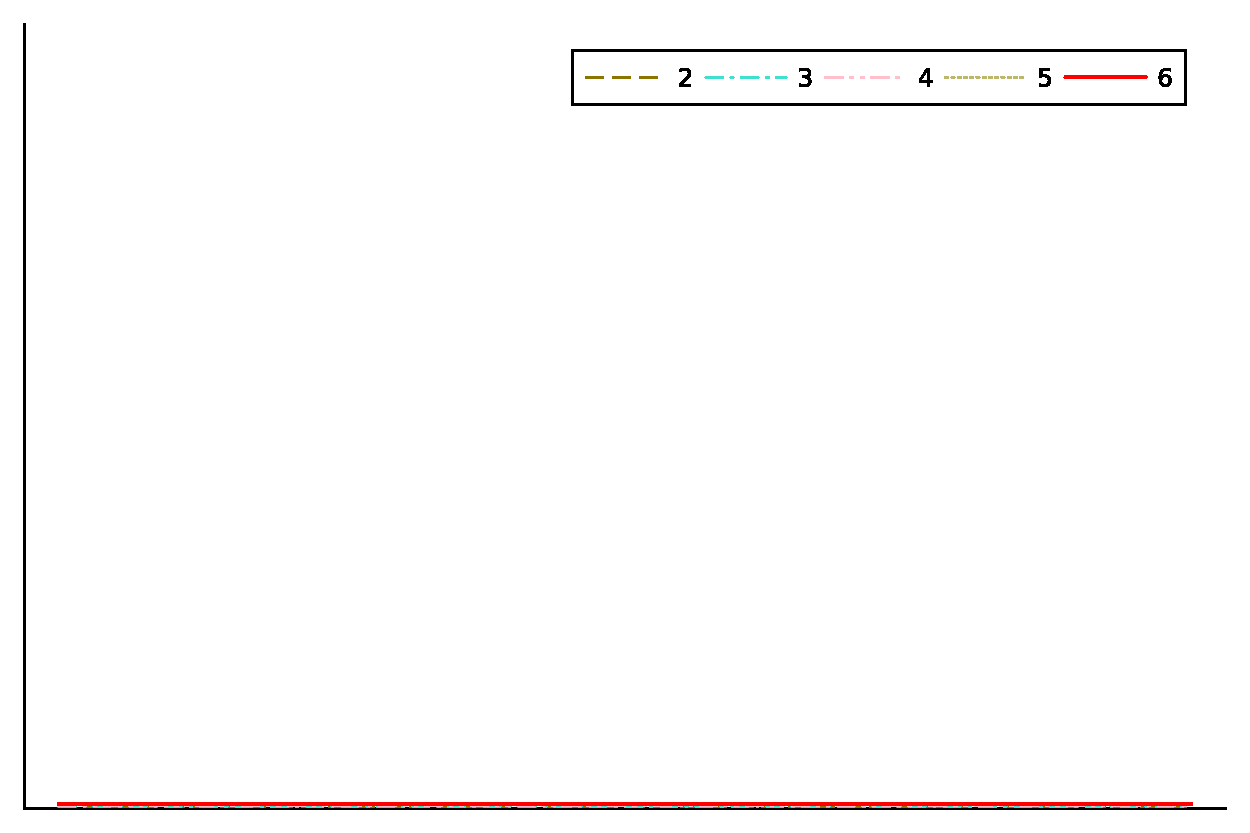
\includegraphics[width=0.4\textwidth,trim={230 340 30 22}, clip]{pdf/pdepics/legends/colors_a-d_new_horiz_2-6_no_order.pdf}\\
	\begin{minipage}[t]{0.32\textwidth}
		\centering
		\includegraphics[width=\textwidth]{pdf/pdepics/disp/IMEXDeC_equispaced_disp_all_2-6_newE.pdf}
		\small$[\DeC, \eq,k,A_k,B_{\lceil k/2 \rceil}]$\par
	\end{minipage}
	\begin{minipage}[t]{0.32\textwidth}
		\centering
		\includegraphics[width=\textwidth]{pdf/pdepics/disp/IMEXDeC_subtimesteps_equispaced_disp_all_2-6_newE.pdf}
		\small$[\sDeC, \eq,k, A_k,B_{\lceil k/2 \rceil}]$\par
	\end{minipage}
	\begin{minipage}[t]{0.32\textwidth}
		\centering
		\includegraphics[width=\textwidth]{pdf/pdepics/disp/IMEXADER_equispaced_disp_all_2-6_newE.pdf}
		\small$[\ADER, \eq,k, A_k,B_{\lceil k/2 \rceil}]$\par
	\end{minipage}\\
	\begin{minipage}[t]{0.32\textwidth}
		\centering
		\includegraphics[width=\textwidth]{pdf/pdepics/disp/IMEXDeC_gaussLobatto_disp_all_2-6_newE.pdf}
		\small$[\DeC, \GLB,k, A_k,B_{\lceil k/2 \rceil}]$\par
	\end{minipage}
	\begin{minipage}[t]{0.32\textwidth}
		\centering
		\includegraphics[width=\textwidth]{pdf/pdepics/disp/IMEXDeC_subtimesteps_gaussLobatto_disp_all_2-6_newE.pdf}
		\small$[\sDeC, \GLB,k, A_k,B_{\lceil k/2 \rceil}]$\par
	\end{minipage}
	\begin{minipage}[t]{0.32\textwidth}
		\centering
		\includegraphics[width=\textwidth]{pdf/pdepics/disp/IMEXADER_gaussLobatto_disp_all_2-6_newE.pdf}
		\small$[\ADER, \GLB,k, A_k,B_{\lceil k/2 \rceil}]$\par
	\end{minipage}
	\caption{Stability areas for orders 2 to 6 with GLB (top) and equi (bottom) nodes, dispersion with stencil $[-\lceil (k+2)/2 \rceil +1 ,\lceil (k+2)/2\rceil]$, advection of order $k$ as in \eqref{eq: r-s_scheme} and time scheme of order $k$}
	\label{fig: disp_allall}
\end{figure}
In Figure~\ref{fig: disp_allall}, we increase all together the order of all operators. In particular, for a given order $k$ for the dispersion operator we use the optimal stencil with support $[-\lceil (k+2)/2 \rceil +1 ,\lceil (k+2)/2\rceil]$, similar to the upwinding of \eqref{eq: shu_upwind_dispersion}. To compute the coefficients of the dispersion operator, we have used the tool \cite{fdcc}. We immediately see that the stability regions shrink and for high order DeC (greater than 5), we lose the stability region $E_P\leq E_{P,0}$. For ADER methods it is even worse, as for high orders (greater than 4) we do not see anymore the stability region $C\leq C_0$ with large $E_P$, while for orders greater than 5 also here the stability region $E_P\leq E_{P,0}$ disappears.


We conclude that the observed IMEX methods combined with the finite difference stencils for the spatial discretization do not possess a spatial-independent condition on the time step (as for the diffusion case). 
Still, in most of the methods a classical stability region for $C\leq C_0$ and $E_P\geq E_{P,1}$, i.e., $P\geq C/E_{P,1}$, is observable, while a time independent stability region for $E_P\leq E_{P,0}$ is present only in few low order cases and it is really linked to the used spatial discretization. 
%at least if we do not use  methods with an A-stable implicit ODE part. 
%For many of the methods with an A-stable implicit ODE part, these lower time step restrictions are so weak that it may not have an effect in many applications, especially because the dispersion coefficient $\beta$ uses to be small, which makes the time step controllable. Nevertheless, we can not rely on this further. 
%The border $C_0$ is also affected by that matter, but because of the really small effects of the afore mentioned methods with the A-stable implicit ODE part, we assume that it does not affect the stability significantly. 
%Moreover, upwind schemes for the dispersion term perform better than central schemes, in terms of stability, while increasing the order of the advection stencils worsen the stability.
%Especially for the ADER methods with order $\le 3$, these stencils show problematic instabilities.
